
\section{Related Work}
\subsection{네트워크 LLM 벤치마크}

Table~\ref{tab:benchmark-comparison}은 기존 네트워크 LLM 벤치마크를 평가 대상별로 정리한 것이다.

\textbf{지식 회상(Knowledge Recall).} LLM이 표준 문서의 내용을 얼마나 정확히 재현하는지를 측정한다. TeleQnA~\cite{ref9}는 3GPP 문서에서 추출한 다지선다 질문으로 통신 도메인 지식을 평가하며, TeleQuAD~\cite{ref10}는 동일 문서에서 구간 추출(Span Extraction) 기반의 읽기 이해를 측정한다. NetBench~\cite{ref11}는 전문가가 큐레이션한 서술형 질문에 대한 LLM의 답변을 전문가 패널이 평가한다. 이들 벤치마크는 LLM의 도메인 지식 보유 여부를 확인하는 데 유용하나, 특정 네트워크 토폴로지에서의 동작을 추론하는 능력은 평가하지 못한다.

\textbf{설정 생성(Configuration Generation).} LLM이 올바른 설정 파일을 작성할 수 있는지를 평가한다. NetConfEval~\cite{wang2024netconfeval}은 주어진 요구 사항으로부터 라우터 설정을 생성하도록 하고, Batfish로 구문 및 의미 정확성을 검증한다. NetComplete~\cite{ref28}은 SMT 기반으로 부분 설정을 자동 완성하는 합성 접근을 제안하였다. NETLLM\allowbreak BENCH~\cite{ref12}는 YANG 스키마 기반의 설정 생성과 에뮬레이션 기반 검증을 결합한다. 이 흐름은 설정 \emph{작성} 능력을 평가하는 반면, 본 연구는 기존 설정을 \emph{읽고 추론}하는 능력에 초점을 맞춘다.

\textbf{동적 추론(Dynamic Reasoning).} 네트워크의 런타임 동작을 추론하는 능력을 평가하며, 본 연구가 속한다. NetPress~\cite{ref7}는 런타임에 네트워크 상태를 생성하고 LLM에게 프로토콜 동작을 예측하도록 하여, 정확도와 안전성을 동시에 측정한다. 본 연구의 전신인 NetConfigQA~\cite{ref26}는 단일 토폴로지에서 설정 해석 QA를 제시하였으나, 인지 난이도 체계와 시뮬레이션 기반 질문(L4/L5)이 부재하였다. NetConfigQA~2.0은 이를 확장하여 \emph{실제 설정 파일}로부터의 5단계 인지 난이도 평가, 4개 토폴로지에 걸친 자동 QA 생성 파이프라인, 그리고 네트워크 데이터에 특화된 평가 지표(TA-Acc)를 제공한다.

\begin{table*}[!t]
  \caption{네트워크 LLM 벤치마크 비교}
  \label{tab:benchmark-comparison}
  \centering
  \small
  \begin{tabular}{|L{3.0cm}|L{2.4cm}|L{2.2cm}|L{2.1cm}|L{2.1cm}|}
    \hline
    \textbf{벤치마크}                        & \textbf{태스크 유형}      & \textbf{데이터 소스}           & \textbf{GT 생성}                 & \textbf{평가 지표}  \\
    \hline
    TeleQnA~\cite{ref9}                  & 지식 회상                & 3GPP 문서                   & 인간+LLM                         & Accuracy        \\
    \hline
    TeleQuAD~\cite{ref10}                & 지식 추출                & 3GPP 규격                   & 구간 추출                          & F1 / EM         \\
    \hline
    NetBench~\cite{ref11}                & 지식 서술                & 전문가                       & 전문가 작성                         & 전문가 평가          \\
    \hline
    NetConfEval~\cite{ref5}              & 설정 생성                & 문서                        & 참조 설정                          & Accuracy        \\
    \hline
    NETLLM\allowbreak BENCH~\cite{ref12} & 생성+검증                & 스키마                       & 에뮬레이션                          & 구문+의미           \\
    \hline
    NetPress~\cite{ref7}                 & 동적 추론                & 런타임 생성                    & 에뮬레이터                          & 정확도+안전          \\
    \hline
    \textbf{Ours}                        & \textbf{설정 해석+동작 추론} & \textbf{실제 \texttt{.cfg}} & \textbf{규칙 기반 + Batfish 시뮬레이션} & \textbf{TA-Acc} \\
    \hline
  \end{tabular}
\end{table*}

\subsection{LLM 기반 네트워크 관리 에이전트}

LLM을 네트워크 운영에 적용하는 연구는 단발성 질의 변환에서 다단계 자율 추론까지 폭넓게 분포한다.

가장 기초적인 형태는 사용자 질문을 도구 전용 쿼리로 번역하는 단발성 접근이다. 대표적으로 AskBatfish~\cite{ref16}는 자연어 질문을 Batfish API 호출로 변환하지만, 다단계 분석이나 도구 간 연계는 지원하지 못하는 한계가 있다.

인텐트 기반 접근은 운영자의 의도를 구체적인 네트워크 설정으로 치환하는 데 집중한다. RAG 기반 에이전트인 INTA~\cite{ref13}는 인텐트를 네트워크 설정으로 치환하여 98.15\%의 높은 구문 정확도를 기록했으며, Confucius~\cite{ref15}는 Multi-Agent 구조를 활용해 인텐트 기반 네트워크 관리의 자동화를 제안한다. 그러나 이러한 연구들은 주로 설정 \emph{작성} 태스크를 다루며, 기존 구성으로부터의 논리적 결론을 도출하는 \emph{추론}은 충분히 다루고 있지 않다.

최근에는 Multi-Agent 구조를 통한 성능 개선 연구가 활발히 진행되고 있다. KubeLLM~\cite{ref14}은 Knowledge Agent와 Tools Agent를 분리하여 단일 에이전트 대비 Kubernetes 관리 정확도를 개선하였다. NIKA~\cite{wang2025network_arena}는 5개 시나리오, 640개 이상의 인시던트를 갖춘 평가 아레나로, MCP 인터페이스를 통해 30개 이상의 도구를 노출하며 GPT-4급 모델의 장애 탐지 능력과 근본 원인 식별의 한계를 보고하였다. 그러나 이 연구들에서 보고된 성능 향상이 에이전트 구조적 설계 덕분인지, 혹은 연결된 도구의 성능 때문인지에 대하나 인과관계는 명확히 분리되지 않았다.

% 본 논문에서 제안하는 NetAlly는 단발성 변환이 아닌 다단계 자율 추론을 수행한다는 점에서 기존 연구와 차별화된다. 에이전트가 토폴로지 분석부터 fork\_snapshot, 차등 도달성 검사, 영향 범위 도출에 이르는 연쇄적 도구 호출을 자율적으로 구성한다. 특히 Batfish(정형 검증), NSO(구성 관리), PNETLab(시뮬레이션)이라는 세 가지의 독립된 관리 평면을 단일 파이프라인에 통합하며, 3-way 비교 실험을 통해 구조와 도구의 기여를 정밀하게 분석한다.



\subsection{연구 위치}
기존 연구는 벤치마크와 시스템 중 하나에 치중된다. TeleQnA, NetConfEval 등은 벤치마크를 제공하지만 한계를 극복할 시스템이 부재하며, 반대로 NIKA, INTA 등은 시스템을 제시하지만 통제된 벤치마크에서의 체계적인 평가가 부족하다.

본 연구는 이 간극을 메우기 위해 벤치마크와 시스템을 하나의 프레임워크로 결합한다. 먼저 NetConfigQA2.0과 TA-Acc로 문제를 정의하고, Single LLM 평가를 통해 한계를 확인한다. 이어서 Pure MAS 실험으로 구조 효과를 분리하고, 도구 통합 시스템 NetAlly를 통해 그 한계를 어떻게 우회할 수 있는지 평가한다. 이 설계를 통해 ``MAS를 도입하면 성능이 향상된다''는 기존 보고를 반복하는 데 그치지 않고, 그 향상의 원천이 구조인지 도구인지까지 분석할 수 있다.

\begin{figure*}[!t]
  \centering
  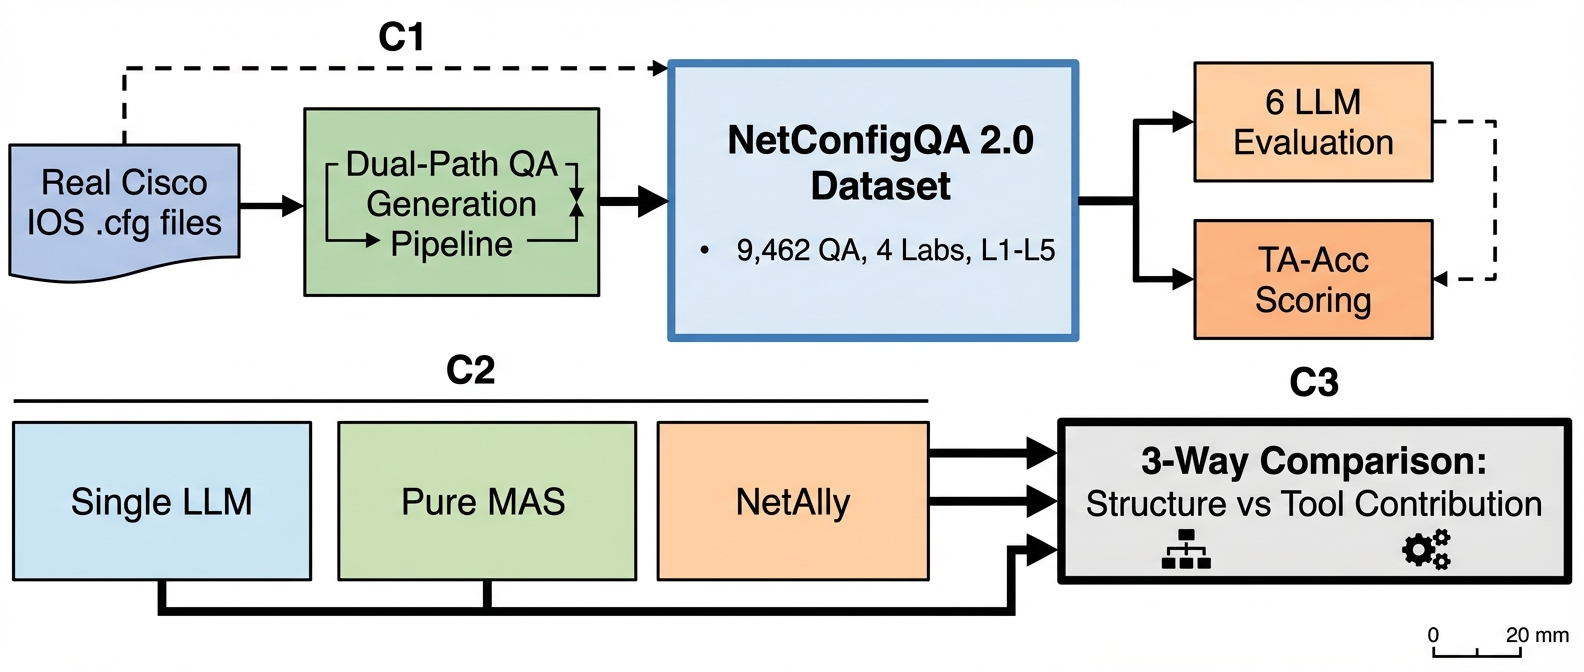
\includegraphics[width=0.7\textwidth]{figure/fig1_framework_overview_ai}
  \caption{연구 프레임워크 개요. 설정 파일로부터 QA를 자동 생성하는 벤치마크와 평가 지표로 LLM의 해석 능력을 평가하고(C1), 이 장벽을 우회하기 위한 도구 통합 시스템을 제시하며(C2), 3-way 비교를 통해 구조 효과와 도구 효과를 분리 분석한다(C3).}
  \label{fig:framework-overview}
\end{figure*}